\begin{footnotesize}
\begin{longtable}{@{}m{.3\textwidth}m{.3\textwidth}m{.05\textwidth}m{.25\textwidth}@{}}
\toprule
\textbf{Außenseite/Oberfläche} & \textbf{Anschliff (Profil)} & \textbf{\textit{Fabric}} & \textbf{Kurzbeschreibung} \\
\midrule
\endhead
\bottomrule
\caption{Keramik: Übersicht über die \textit{Fabrics}.}
\label{tab:Fabrics_Bilder}
\endfoot
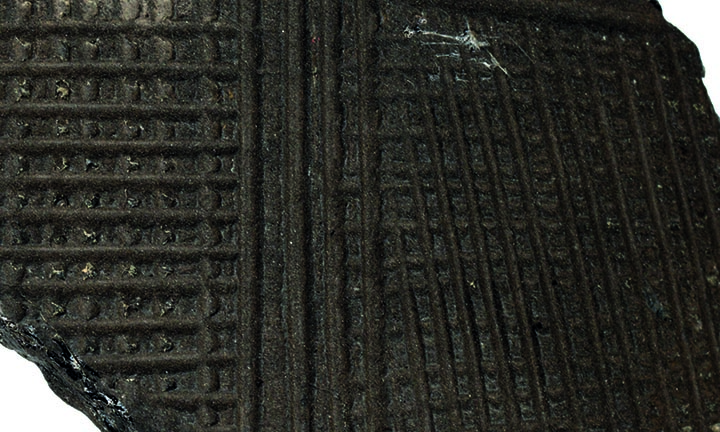
\includegraphics[width=.3\textwidth]{misc/Systematik/Fabrics/Obfl/PIK87-1-8-6_aussen_5cm.jpg} & 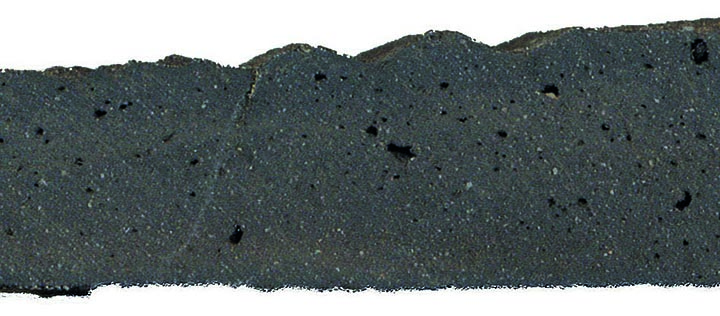
\includegraphics[width=.3\textwidth]{misc/Systematik/Fabrics/Prof/PIK87-1I9-1_2cm.jpg} & 1a & Der \textit{Scherben} lässt makroskopisch keine nichtplastischen Partikel erkennen und ist im Anschliff komplett schwarz (Obj.:~PIK~87/1/I-9:1). \\
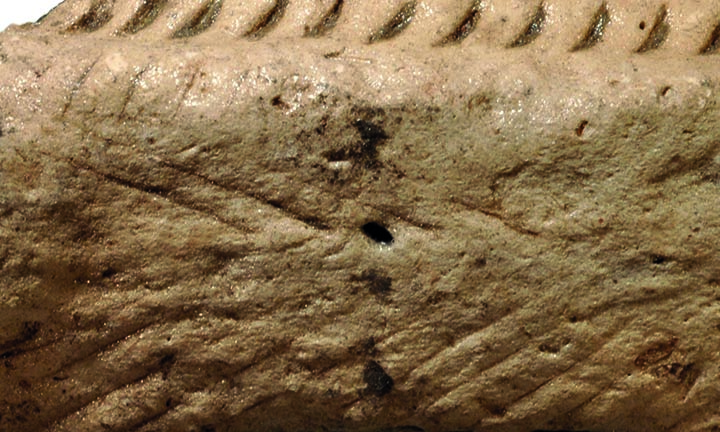
\includegraphics[width=.3\textwidth]{misc/Systematik/Fabrics/Obfl/MBA_201-12_5cm.jpg} & 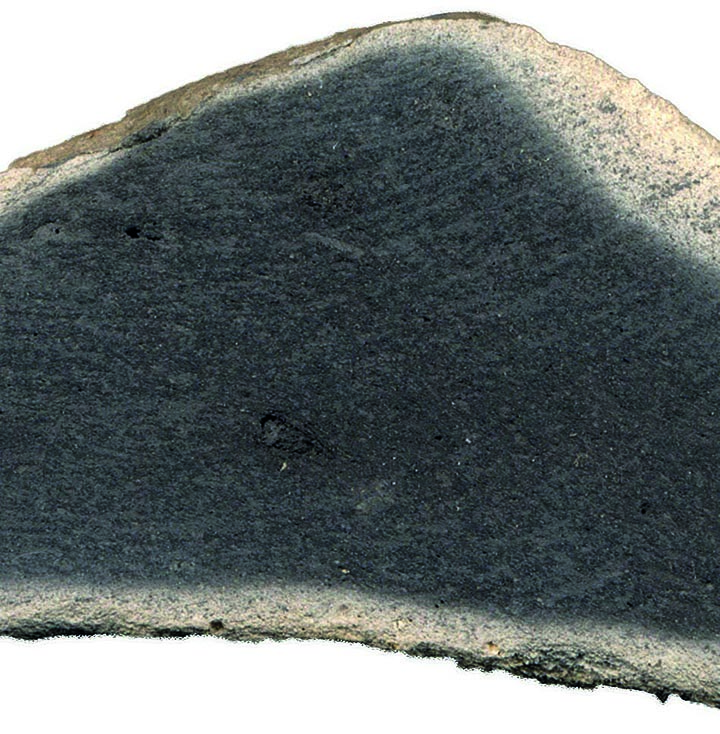
\includegraphics[width=.3\textwidth]{misc/Systematik/Fabrics/Prof/MBA_201-12_2cm.jpg} & 1b & Wie 1a, der \textit{Scherben} ist jedoch randlich weißbrennend oxidiert. Der Bereich der Oxidation lässt sich deutlich vom dunklen Kern abgrenzen (Obj.:~MBA~201:12). \\
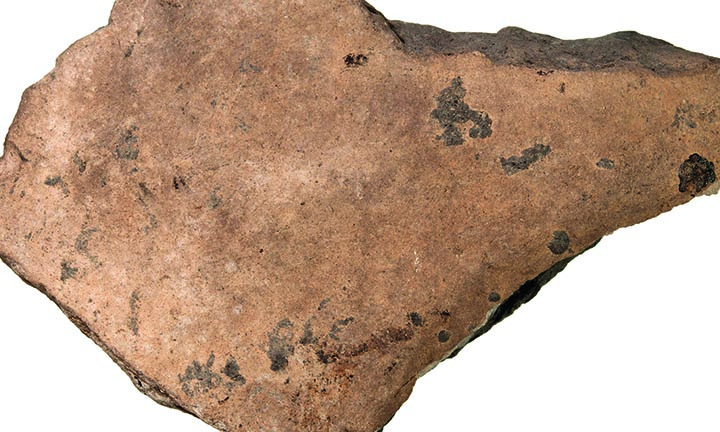
\includegraphics[width=.3\textwidth]{misc/Systematik/Fabrics/Obfl/MSN87-101-142_5cm.jpg} & 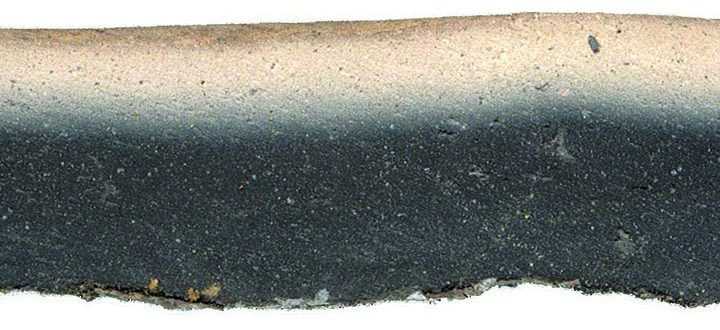
\includegraphics[width=.3\textwidth]{misc/Systematik/Fabrics/Prof/MSN87-101-142_2cm.jpg} & 1c & Wie 1a, der \textit{Scherben} ist jedoch auf einer Seite deutlich oxidiert, während auf der Gegenseite keine Oxidation sichtbar ist. Der oxidierte Bereich grenzt sich scharf vom dunklen Kern ab (Obj.:~MSN~87/101:142).\vspace{1em} \\
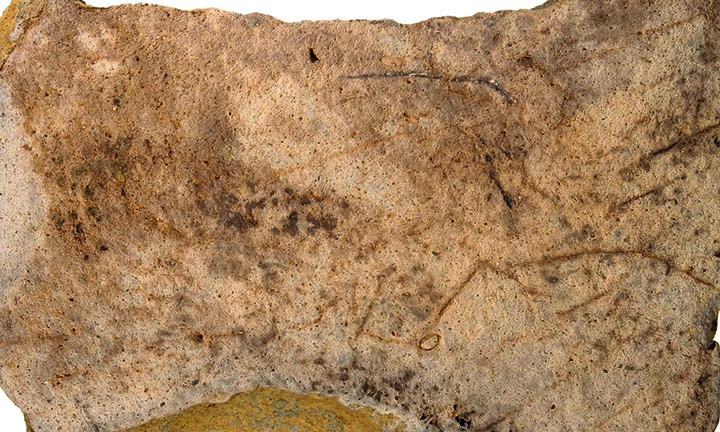
\includegraphics[width=.3\textwidth]{misc/Systematik/Fabrics/Obfl/BTW87-101-43_5cm.jpg} & 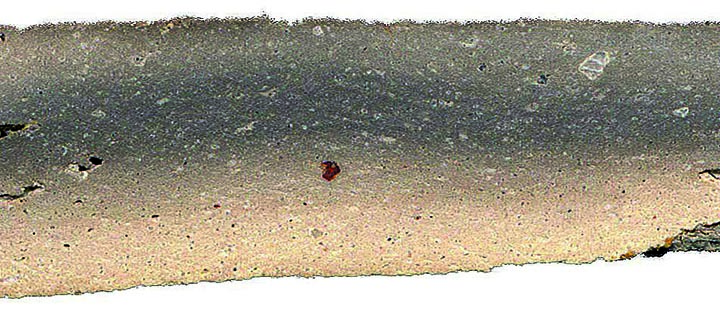
\includegraphics[width=.3\textwidth]{misc/Systematik/Fabrics/Prof/BTW87-101-43_2cm.jpg} & 1d & Wie 1a, der \textit{Scherben} ist jedoch größtenteils, bis auf einen teilweise nur blassen, dunklen Restkern oxidiert. Die oxidierte Zone geht fließend in den Restkern über (Obj.:~BTW~87/101:43). \\
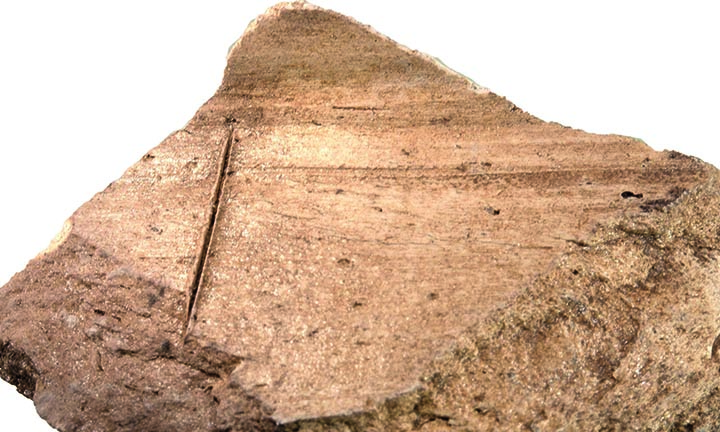
\includegraphics[width=.3\textwidth]{misc/Systematik/Fabrics/Obfl/IKE81-1-12_5cm.jpg} & 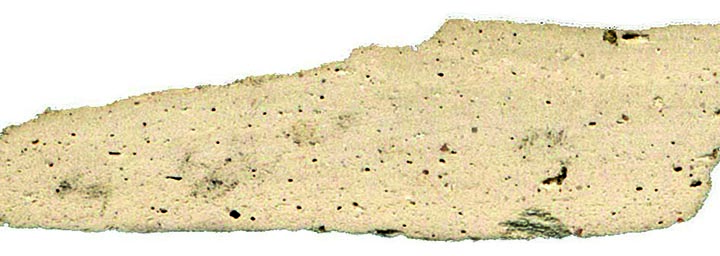
\includegraphics[width=.3\textwidth]{misc/Systematik/Fabrics/Prof/IKE81-1-12_2cm.jpg} & 1e & Wie 1a, der \textit{Scherben} ist jedoch vollständig durchoxidiert, ein Kern ist nicht mehr zu beobachten (Obj.:~IKE~81/1:12). \\
% *** MAßSTAB ***
\includegraphics[width=.3\textwidth, page = 1]{misc/Systematik/Fabrics/fabrics_scales.pdf} & \includegraphics[width=.3\textwidth, page = 2]{misc/Systematik/Fabrics/fabrics_scales.pdf} &  &  \\
% *** MAßSTAB ***
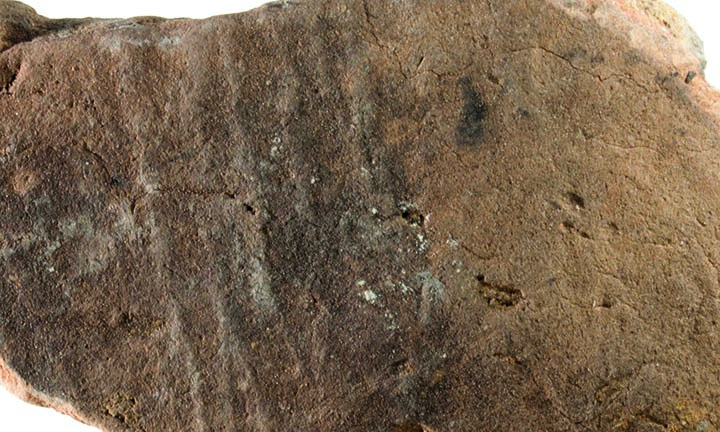
\includegraphics[width=.3\textwidth]{misc/Systematik/Fabrics/Obfl/BKE81-2-2-9_5cm.jpg} & 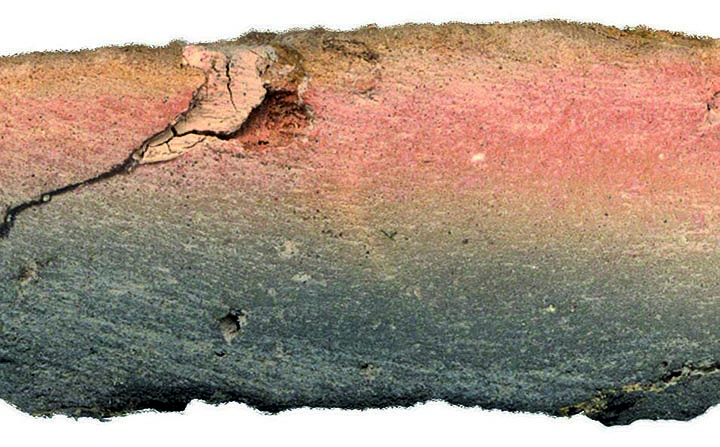
\includegraphics[width=.3\textwidth]{misc/Systematik/Fabrics/Prof/BKE81-2-2-9_2cm.jpg} & 2a & Wie 1d, jedoch ist der genutzte Ton rotbrennend. Ein Restkern ist noch sichtbar (Obj.:~BKE~81/2-2:9). \\
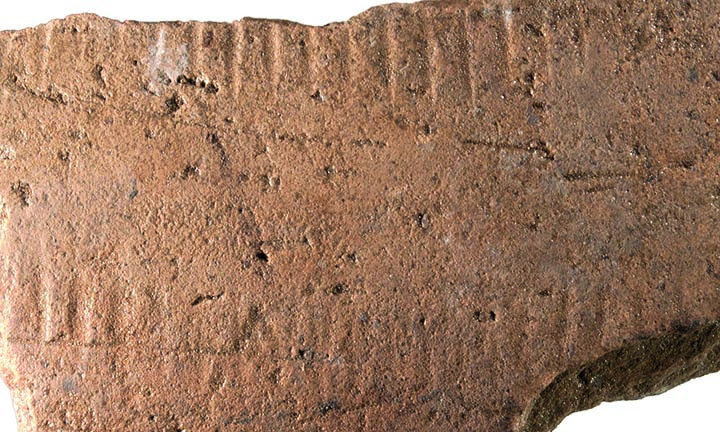
\includegraphics[width=.3\textwidth]{misc/Systematik/Fabrics/Obfl/IMB81-3-2_11_5cm.jpg} & 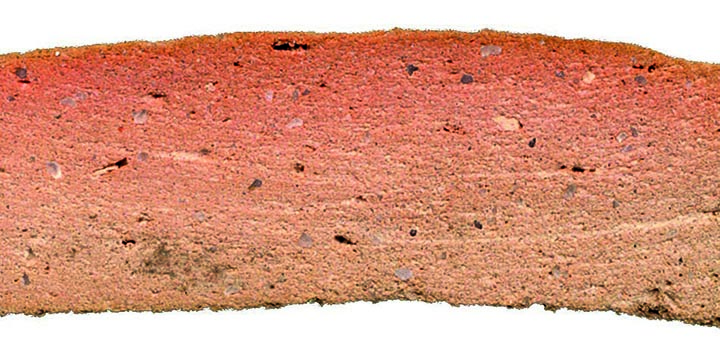
\includegraphics[width=.3\textwidth]{misc/Systematik/Fabrics/Prof/IMB81-3-2_11_2cm.jpg} & 2b & Wie 2a, der \textit{Scherben} ist vollständig rotbrennend durchoxidiert (Obj.:~IMB~81/3-2:11). \\
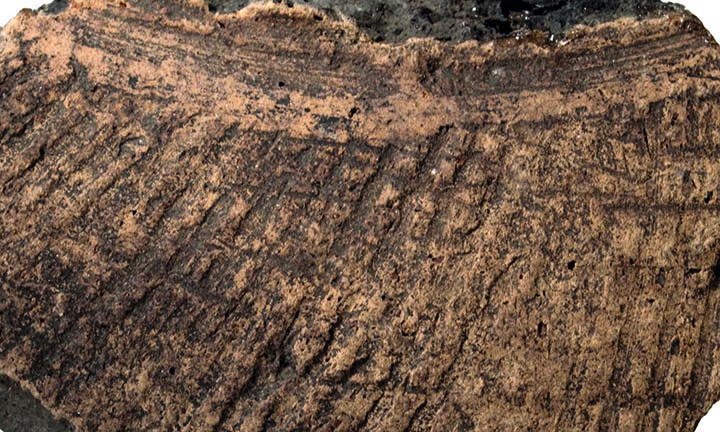
\includegraphics[width=.3\textwidth]{misc/Systematik/Fabrics/Obfl/PIK87-1-2-225_5cm.jpg} & 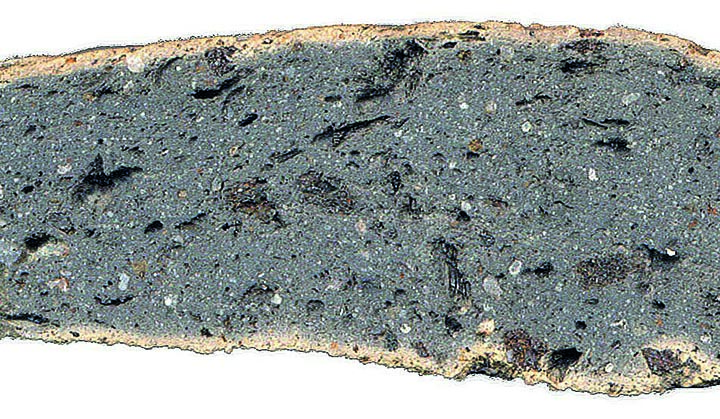
\includegraphics[width=.3\textwidth]{misc/Systematik/Fabrics/Prof/PIK87-1-2-225_2cm.jpg} & 3a & Der \textit{Scherben} enthält bis zu 20~\% nichtplastische Partikel der Größenklassen \textit{medium} bis \textit{coarse} (250--1000\,$\mu$m) und zeigt innen wie außen eine schmale, scharf abzugrenzende, weißbrennende Oxidationszone. In geringem Maße finden sich ausgebrannte Reste organischer Partikel (Obj.:~PIK~87/1-2:225). \\
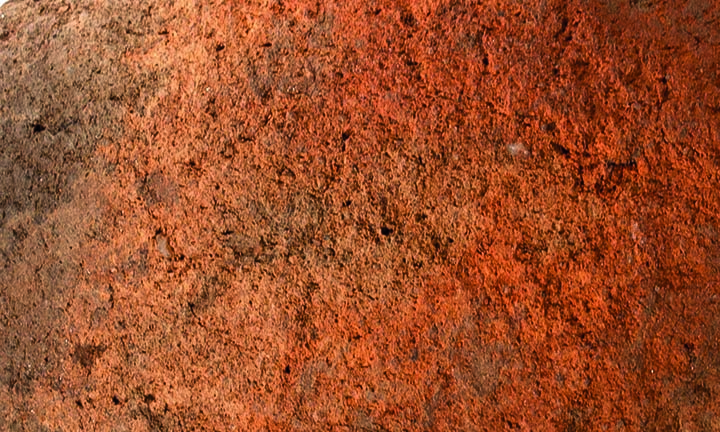
\includegraphics[width=.3\textwidth]{misc/Systematik/Fabrics/Obfl/PDM87-102-20_5cm.jpg} & 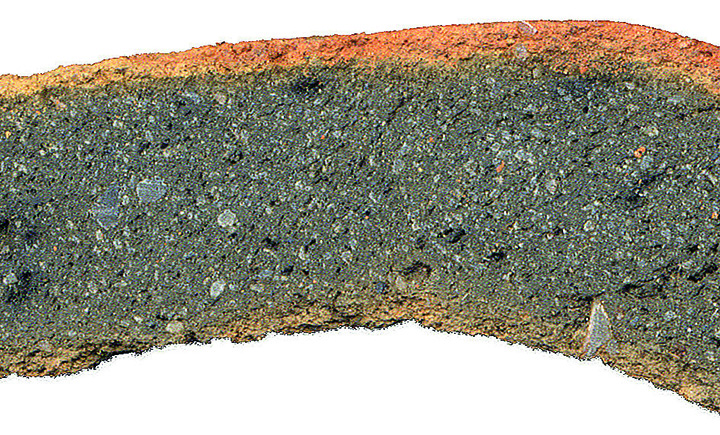
\includegraphics[width=.3\textwidth]{misc/Systematik/Fabrics/Prof/PDM87-102-20_2cm.jpg} & 3b & Wie 3a, die Brennfarbe des Scherbens ist rot (Obj.:~PDM~87/102:20). \\
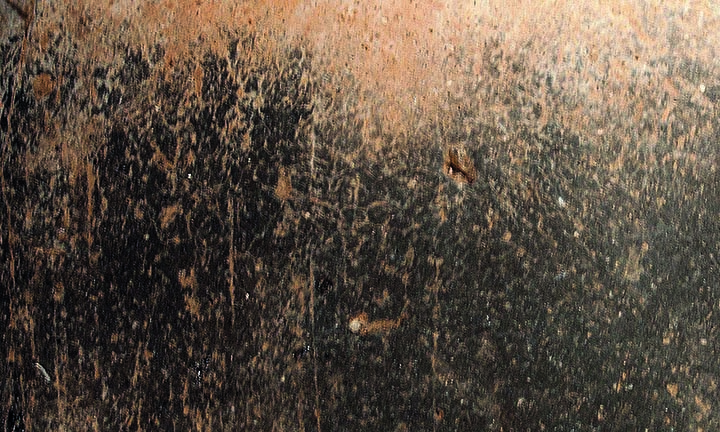
\includegraphics[width=.3\textwidth]{misc/Systematik/Fabrics/Obfl/BYN87-101-10_5cm.jpg} & 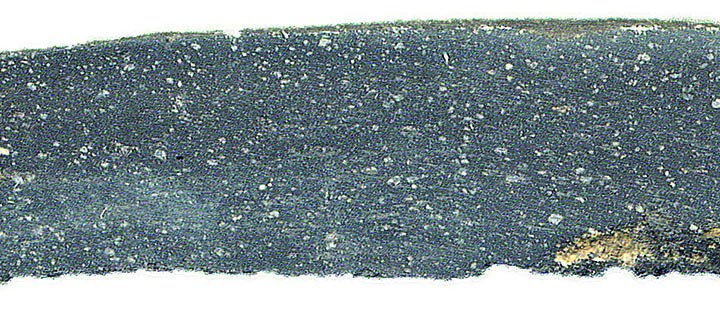
\includegraphics[width=.3\textwidth]{misc/Systematik/Fabrics/Prof/BYN87-101-10_2cm.jpg} & 3c & Wie 3a, der \textit{Scherben} zeigt keine randliche Oxidation. Hinweise auf ausgebrannte Organik sind sehr selten (Obj.:~BYN~87/101:10). \\
% *** MAßSTAB ***
\includegraphics[width=.3\textwidth, page = 1]{misc/Systematik/Fabrics/fabrics_scales.pdf} & \includegraphics[width=.3\textwidth, page = 2]{misc/Systematik/Fabrics/fabrics_scales.pdf} &  &  \\
% *** MAßSTAB ***
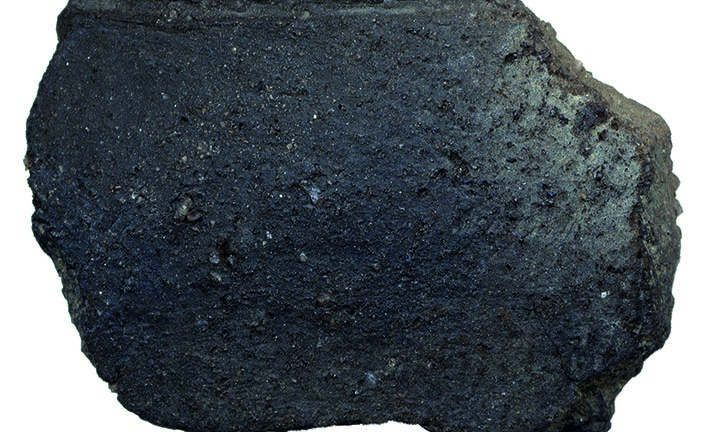
\includegraphics[width=.3\textwidth]{misc/Systematik/Fabrics/Obfl/PIK87-1-8-1_5cm.jpg} & 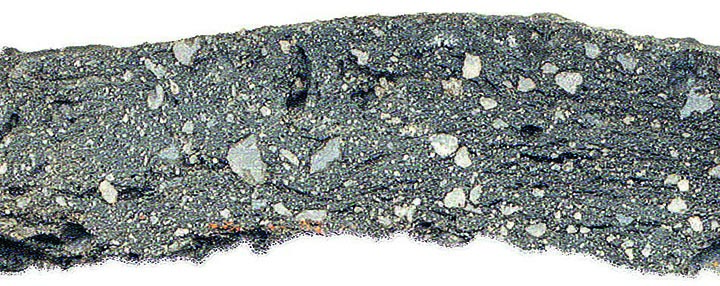
\includegraphics[width=.3\textwidth]{misc/Systematik/Fabrics/Prof/PIK87-1-8-1_2cm.jpg} & 4a & Der \textit{Scherben} enthält bis zu 40~\% nichtplastischer Partikel (kantiger Quarz) der Größenklassen \textit{coarse} bis \textit{very coarse} (500--2000\,$\mu$m). Im Anschliff ist er komplett grau bis schwarz (Obj.:~PIK~87/1-8:1).\vspace{1em} \\
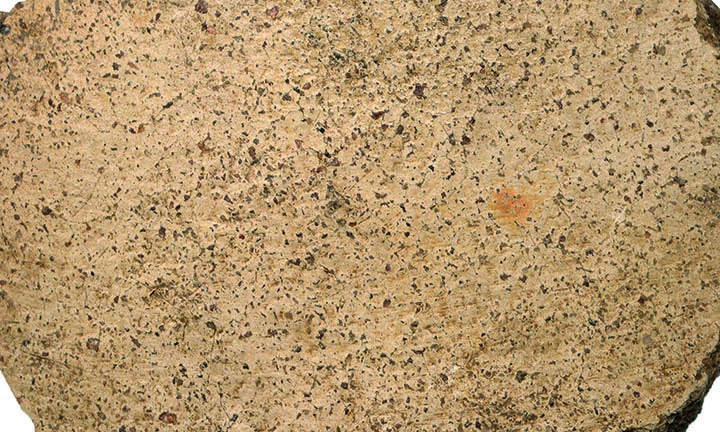
\includegraphics[width=.3\textwidth]{misc/Systematik/Fabrics/Obfl/DON85-102-1_5cm.jpg} & 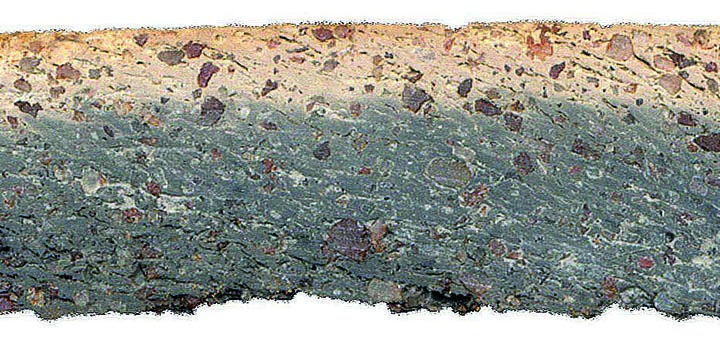
\includegraphics[width=.3\textwidth]{misc/Systematik/Fabrics/Prof/DON85-102-1_2cm.jpg} & 4b & Wie 4a, teilweise enthält der \textit{Scherben} rötliche, leicht abgerundete Quarzkörner. Regelhaft weist er eine gut abzugrenzende, weißbrennende Oxidationszone auf (Obj.:~DON~85/102:1).\vspace{1em} \\
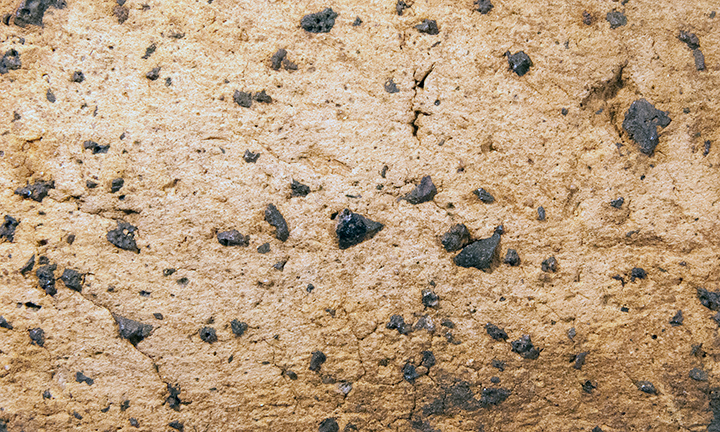
\includegraphics[width=.3\textwidth]{fabrics/surf_5cm/Mukila_62062_DSC_4829.jpg} & 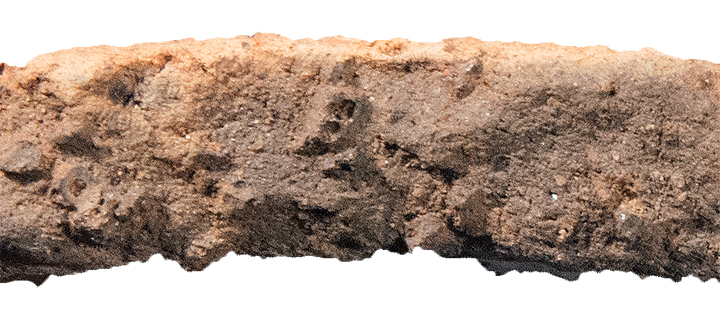
\includegraphics[width=.3\textwidth]{fabrics/surf_5cm/Mukila_62062_DSC_4835.jpg} & 4b.1 & Wie 4b, nichplastische Partikel sind zerstoßene Schlacken (Obj.:~Mukila 1952 Inv.-Nr.~62062).\vspace{1em} \\
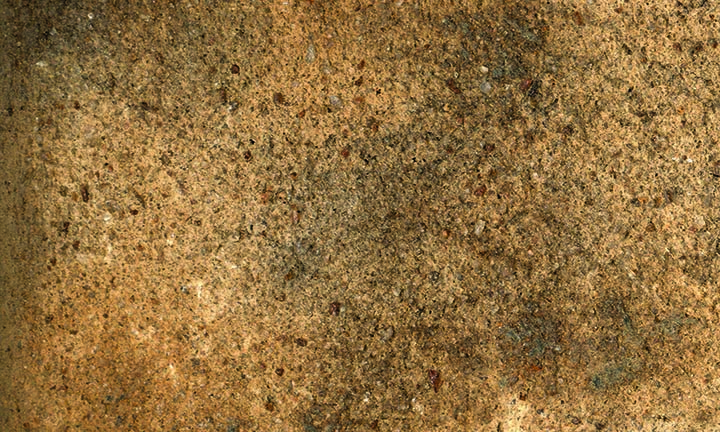
\includegraphics[width=.3\textwidth]{misc/Systematik/Fabrics/Obfl/MBN85-101-60_5cm.jpg} & 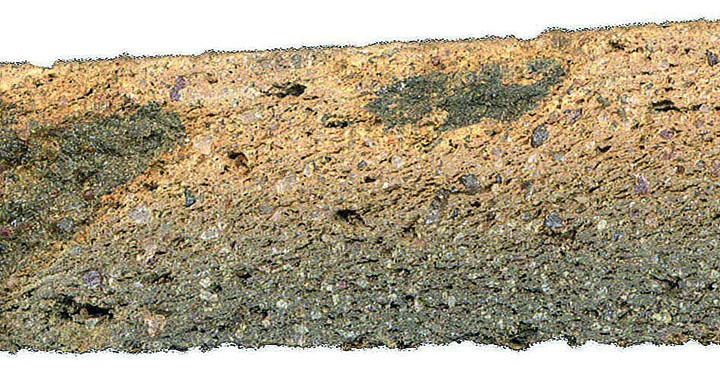
\includegraphics[width=.3\textwidth]{misc/Systematik/Fabrics/Prof/MBN85-101-60_2cm.jpg} & 4c & Wie 4a, der \textit{Scherben} ist bis auf einen meist schwachen Restkern deutlich weißbrennend oxidiert. Die Grenze zum Restkern ist nur schwach ausgeprägt (Obj.: MBN 85/101:60). \\
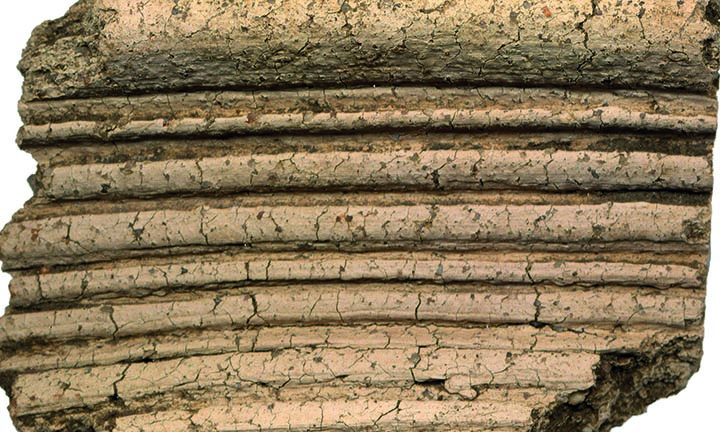
\includegraphics[width=.3\textwidth]{misc/Systematik/Fabrics/Obfl/MLB85-101-22_5cm.jpg} & 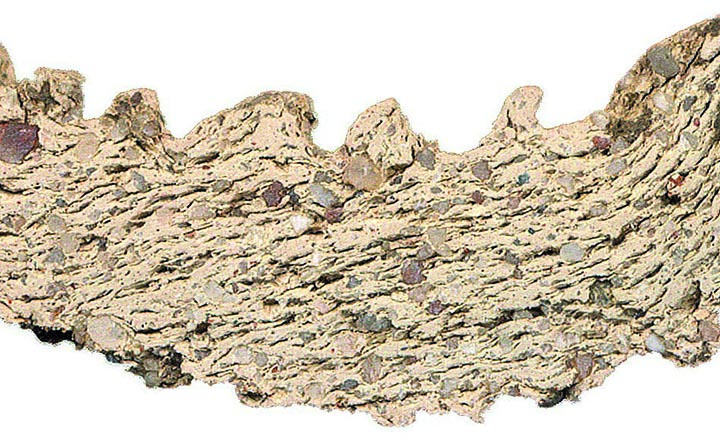
\includegraphics[width=.3\textwidth]{misc/Systematik/Fabrics/Prof/MLB85-101-22_2cm.jpg} & 4d & Wie 4a, der \textit{Scherben} ist vollständig weißbrennend durchoxidiert (Obj.:~MLB~85/101:22). \\
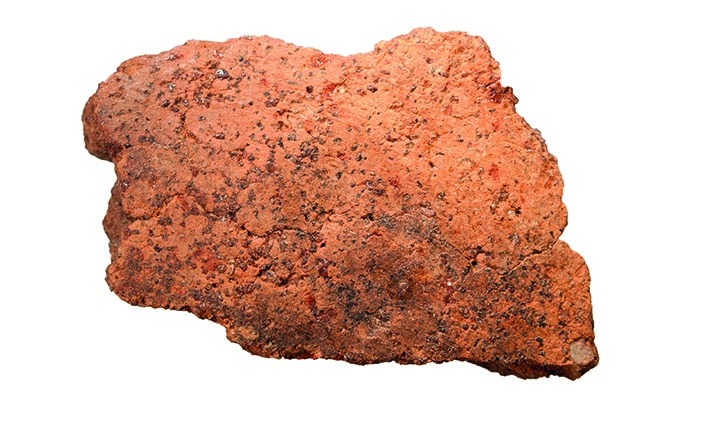
\includegraphics[width=.3\textwidth]{misc/Systematik/Fabrics/Obfl/MTB85-101-101_5cm.jpg} & 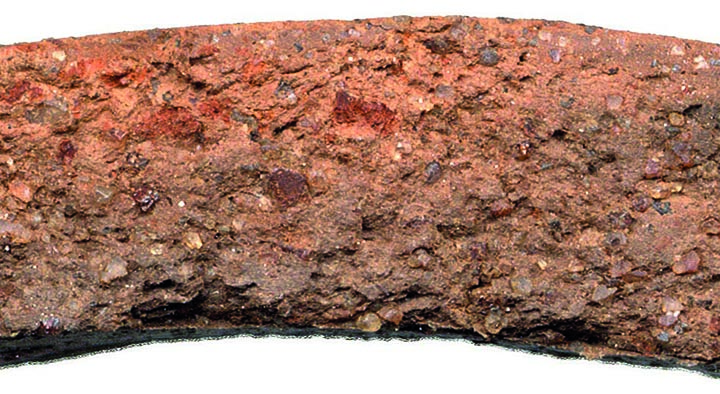
\includegraphics[width=.3\textwidth]{misc/Systematik/Fabrics/Prof/MTB85-101-101_2cm.jpg} & 5a & Wie 4a, der \textit{Scherben} ist vollständig rotbrennend oxidiert (Obj.:~MTB~85/101:101). \\
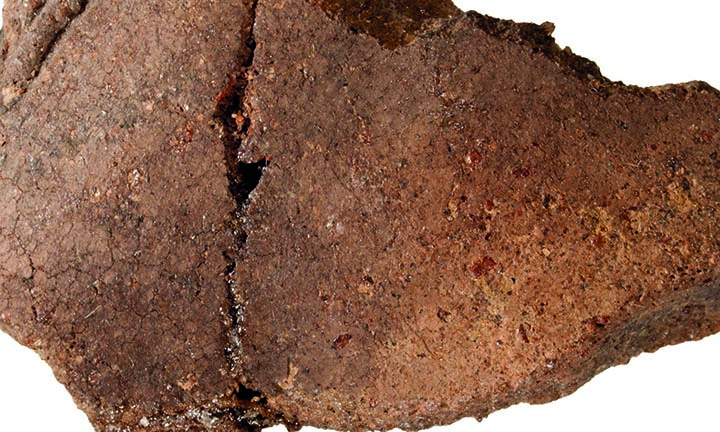
\includegraphics[width=.3\textwidth]{misc/Systematik/Fabrics/Obfl/DON85-102-123_5cm.jpg} & 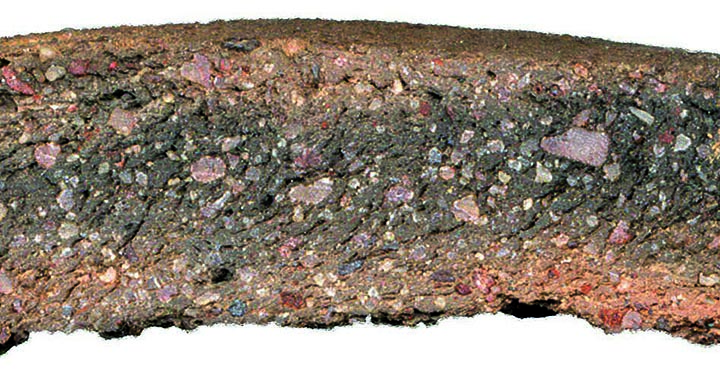
\includegraphics[width=.3\textwidth]{misc/Systematik/Fabrics/Prof/DON85-102-123_2cm.jpg} & 5b & Wie 5a, der \textit{Scherben} ist bis auf einen nur schwach abzugrenzenden, dunklen Restkern rotbrennend oxidiert (Obj.:~DON~85/102:123). \\
% *** MAßSTAB ***
\includegraphics[width=.3\textwidth, page = 1]{misc/Systematik/Fabrics/fabrics_scales.pdf} & \includegraphics[width=.3\textwidth, page = 2]{misc/Systematik/Fabrics/fabrics_scales.pdf} &  &  \\
% *** MAßSTAB ***
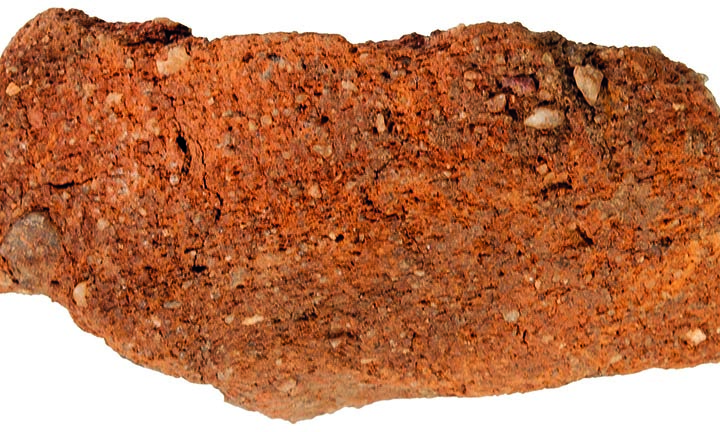
\includegraphics[width=.3\textwidth]{misc/Systematik/Fabrics/Obfl/OUE87-102-49_5cm.jpg} & 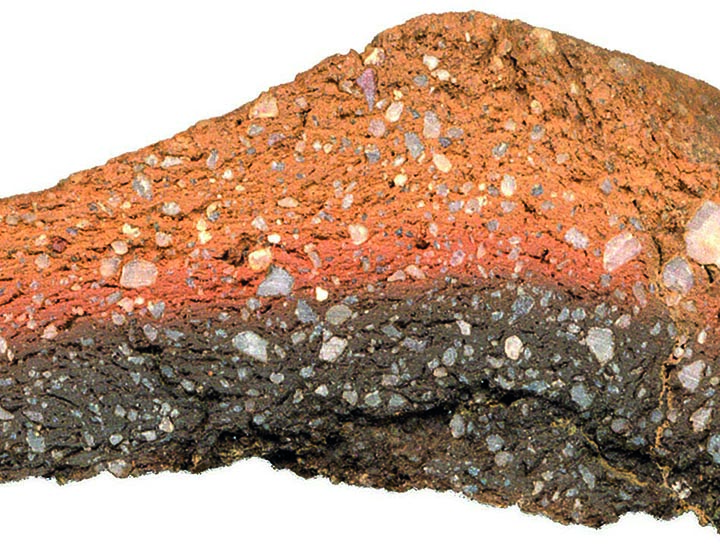
\includegraphics[width=.3\textwidth]{misc/Systematik/Fabrics/Prof/OUE87-102-49_2cm.jpg} & 5c & Wie 5a, der \textit{Scherben} weist eine scharf abzugrenzenden rotoxidierte Zone auf (Obj.:~OUE~87/102:49). \\
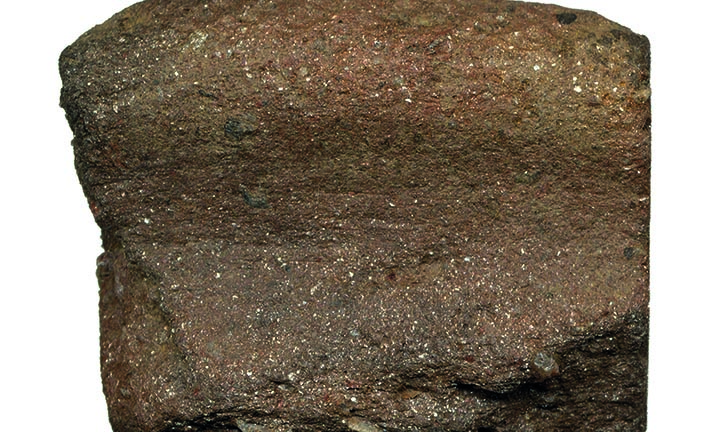
\includegraphics[width=.3\textwidth]{misc/Systematik/Fabrics/Obfl/SID85-101-2_5cm.jpg} & 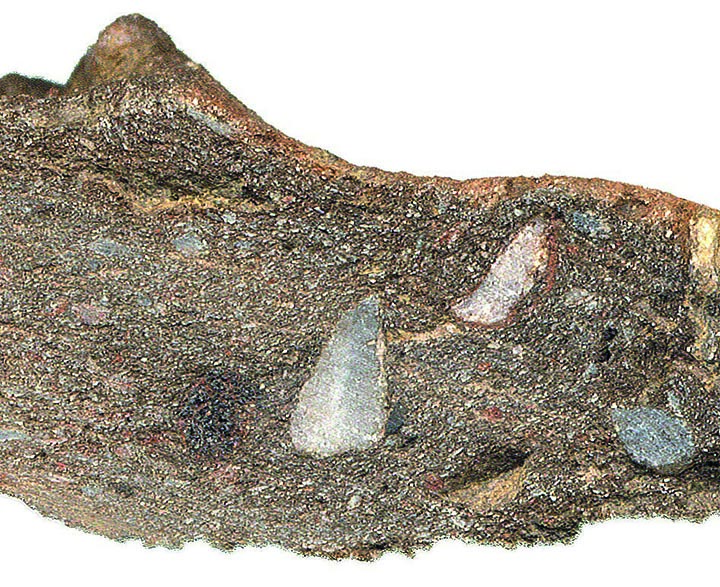
\includegraphics[width=.3\textwidth]{misc/Systematik/Fabrics/Prof/SID85-101-2_2cm.jpg} & 6a & Der \textit{Scherben} enthält neben bis zu 40~\% kantigem Quarz der Größenklassen \textit{fine} bis \textit{very coarse} (125--2000\,$\mu$m) auffällig glimmerartiges Material (Obj.: SID 85/101:2). \\
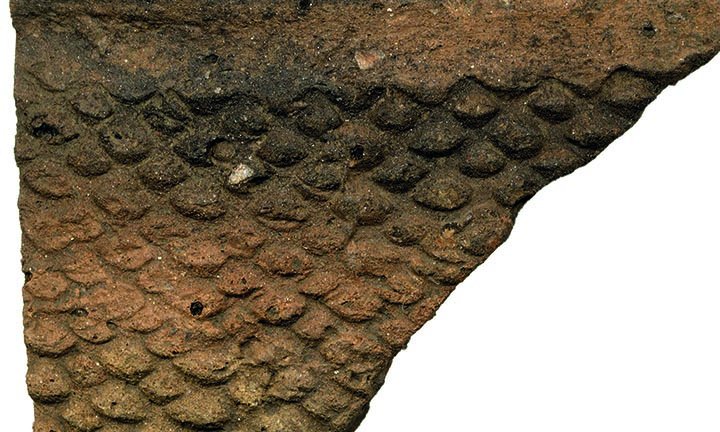
\includegraphics[width=.3\textwidth]{misc/Systematik/Fabrics/Obfl/KOU85-101-59_5cm.jpg} & 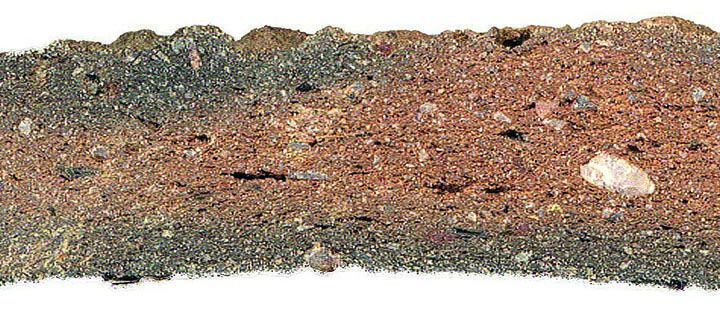
\includegraphics[width=.3\textwidth]{misc/Systematik/Fabrics/Prof/KOU85-101-59_2cm.jpg} & 6b & Wie 6b, die Farbe des \textit{Scherbens} schwankt zwischen rot, braun und grau (Obj.:~KOU~85/101:59). \\
 & & 6c & Wie 6b, jedoch aus eine aufällig weiß-brennenden Ton(Obj.:~YEA~01/10/27/8). \\
 & & 6d & Wie 6b, jedoch mit deutlich scharfer Oxidationsgrenze (siehe 1b) (Obj.:~YEA~10). \\
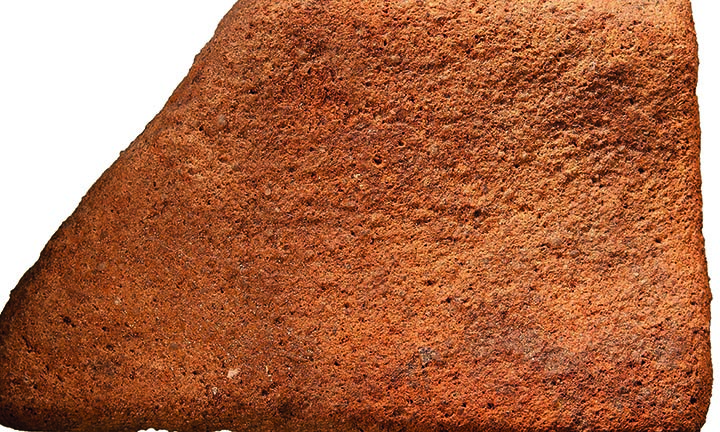
\includegraphics[width=.3\textwidth]{misc/Systematik/Fabrics/Obfl/BNA87-101-3_5cm.jpg} & 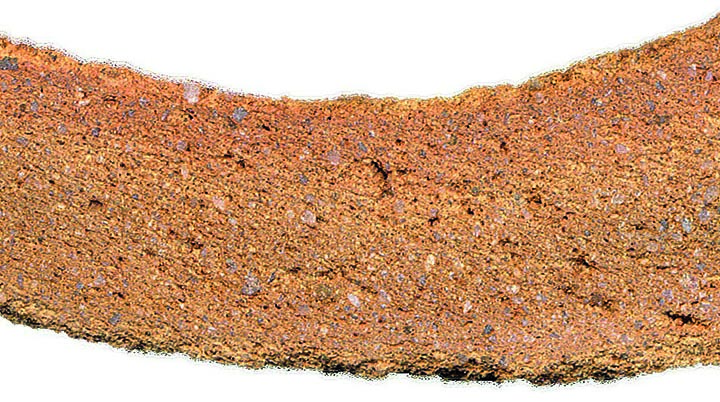
\includegraphics[width=.3\textwidth]{misc/Systematik/Fabrics/Prof/BNA87-101-3_2cm.jpg} & 7a & Der \textit{Scherben} enthält bis zu 10~\% Quarzkörner der Größenklassen \textit{fine} bis \textit{coarse} (125--1000\,$\mu$m). Das Stück ist komplett rotbrennend durchoxidiert (Obj.:~BNA~87/101:3).\vspace{1em} \\
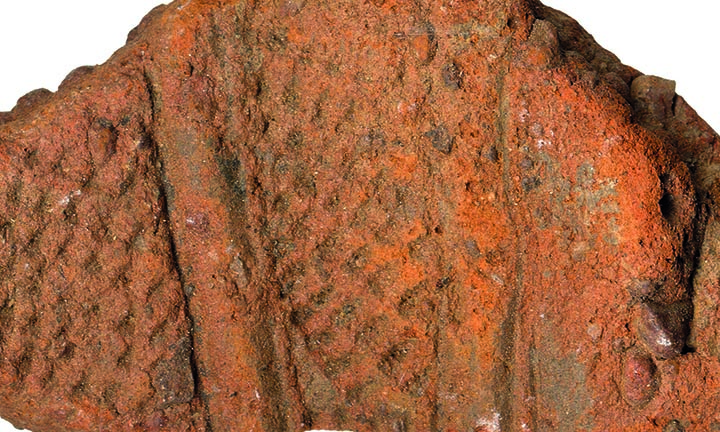
\includegraphics[width=.3\textwidth]{misc/Systematik/Fabrics/Obfl/BMS87-101-1_5cm.jpg} & 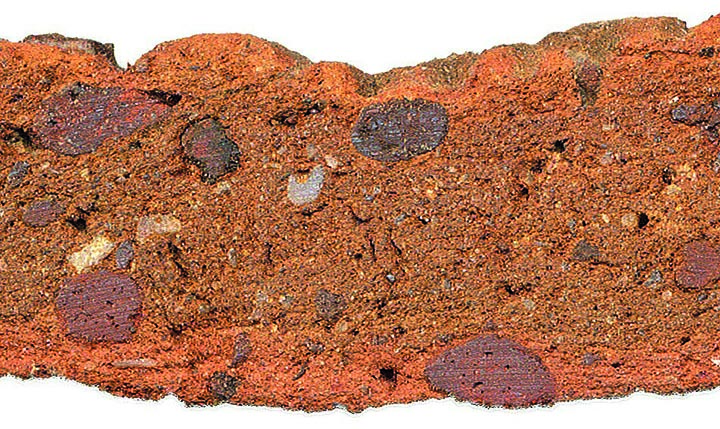
\includegraphics[width=.3\textwidth]{misc/Systematik/Fabrics/Prof/BMS87-101-1_2cm.jpg} & 7b & Wie 7a, der \textit{Scherben} enthält neben Quarzkörnern auch häufig abgerundete, an Laterit erinnernde Partikel der Größenklassen \textit{coarse} bis \textit{very coarse} (500--2000\,$\mu$m). (Obj.:~BMS~87/101:1). \\
% *** MAßSTAB ***
\includegraphics[width=.3\textwidth, page = 1]{misc/Systematik/Fabrics/fabrics_scales.pdf} & \includegraphics[width=.3\textwidth, page = 2]{misc/Systematik/Fabrics/fabrics_scales.pdf} &  &  \\
% *** MAßSTAB ***
\includegraphics[width=.3\textwidth]{misc/Systematik/Fabrics/Obfl/MBK85-101-81_5cm.jpg} & \includegraphics[width=.3\textwidth]{misc/Systematik/Fabrics/Prof/MBK85-101-81_2cm.jpg} & 7c & Wie 7a, der \textit{Scherben} enthält neben Quarz und kleineren Stücken lateritartigen Materials auch eine an Glimmer erinnernde Fraktion feiner Partikel (Obj.:~MBK~85/101:81).\vspace{1em} \\
\includegraphics[width=.3\textwidth]{misc/Systematik/Fabrics/Obfl/MLB85-1-1-87_5cm.jpg} & \includegraphics[width=.3\textwidth]{misc/Systematik/Fabrics/Prof/MLB85-1-1-87_2cm.jpg} & 7d & Wie 7a, der \textit{Scherben} zeigt eine von einem grauen bis schwarzen Kern scharf abgrenzbare, rotbrennende Oxidation (Obj.:~MLB~85/1-1:87).\vspace{1em} \\
\includegraphics[width=.3\textwidth]{misc/Systematik/Fabrics/Obfl/MND85-101-21_5cm.jpg} & \includegraphics[width=.3\textwidth]{misc/Systematik/Fabrics/Prof/MND85-101-21_2cm.jpg} & 7e & Wie 7d, der \textit{Scherben} zeigt einen homogen grauen Kern mit einer scharf abgegrenzten, nur wenige Millimeter tief eindringenden, rotbrennenden Oxidation. Neben feinen Quarzkörnern enthält er lateritartige Partikel der Größenklassen \textit{coarse} bis \textit{very coarse} (500--2000\,$\mu$m) (Obj.:~MND~85/101:21).\vspace{1em} \\
\includegraphics[width=.3\textwidth]{misc/Systematik/Fabrics/Obfl/KPT85-101-9_5cm.jpg} & \includegraphics[width=.3\textwidth]{misc/Systematik/Fabrics/Prof/KPT85-101-9_2cm.jpg} & 8a & Der \textit{Scherben} enthält neben Quarzkörnern, Resten ausgebrannter Organik sowie teilweise glimmerartigen Partikeln auch eine Fraktion Schamott. Die Zusammensetzung der nichtplastischen Partikel ist mit Bezug auf Art, Größe und Dichte sehr heterogen (Obj.:~KPT~85/101:9). \\
% *** MAßSTAB ***
\includegraphics[width=.3\textwidth, page = 1]{misc/Systematik/Fabrics/fabrics_scales.pdf} & \includegraphics[width=.3\textwidth, page = 2]{misc/Systematik/Fabrics/fabrics_scales.pdf} &  &  \\
% *** MAßSTAB ***
\includegraphics[width=.3\textwidth]{misc/Systematik/Fabrics/Obfl/SUN87-101-72_5cm.jpg} & \includegraphics[width=.3\textwidth]{misc/Systematik/Fabrics/Prof/SUN87-101-72_2cm.jpg} & 9a & Der Scherben enthält ausschließlich Schamott der Größenklassen \textit{coarse} bis \textit{very coarse} (500--2000\,$\mu$m). Ein grauer bis schwarzer Kern wird von einer scharf abzugrenzenden, randlichen, weißbrennenden Oxidationszone umschlossen (Obj.:~SUN~87/101:72).\vspace{1em} \\
\includegraphics[width=.3\textwidth]{misc/Systematik/Fabrics/Obfl/SUN87-101-87_5cm.jpg} & \includegraphics[width=.3\textwidth]{misc/Systematik/Fabrics/Prof/SUN87-101-87_2cm.jpg} & 9b & Wie 9a, der \textit{Scherben} ist vollständig weißbrennend durchoxidiert (Obj.:~SUN~87/101:87) \\
% *** MAßSTAB ***
\includegraphics[width=.3\textwidth, page = 1]{misc/Systematik/Fabrics/fabrics_scales.pdf} & \includegraphics[width=.3\textwidth, page = 2]{misc/Systematik/Fabrics/fabrics_scales.pdf} &  &  \\
% *** MAßSTAB ***
\end{longtable}
\end{footnotesize}